Um die News zu bearbeiten, klicken Sie im \enquote{Data-Input-Menu} auf den Punkt \enquote{News hinzufügen}
\\
\begin{figure}[H]
\centering
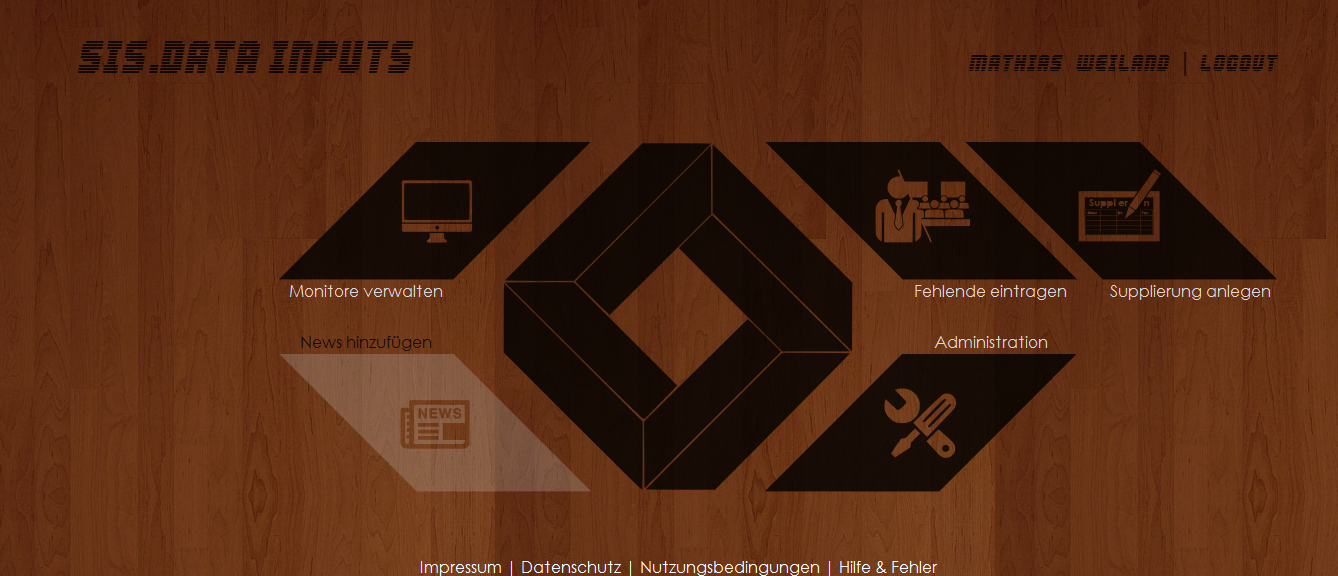
\includegraphics[keepaspectratio=true, width=16cm]{images/screenshots/data-inputs_news.png}
\caption{Data-Input-Menü}
\label{fig:instr_admin_data_inputs_news}
\end{figure}


Nach dem Öffnen der Seite werden die eingetragenen News angezeigt.
\\

\subsection{News bearbeiten/hinzufügen}

\begin{figure}[H]
\centering
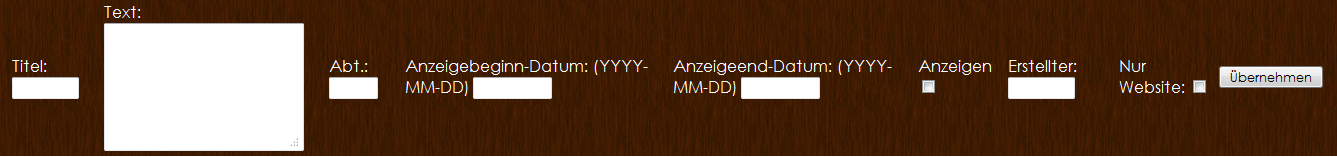
\includegraphics[keepaspectratio=true, width=16cm]{images/screenshots/news_inserts.png}
\caption{News eintragen}
\label{fig:instr_admin_news_insert}
\end{figure}


\begin{description} 
\item[Titel] Titel der angezeigt werden soll.
\item[Text] Text der angezeigt werden soll.
\item[Abt.] Abteilung für welche die News angezeigt werden soll. Wenn dieses Feld leer ist, wird die News in allen Abteilungen angezeigt.
\item[Anzeigebeginn-Datum] Datum ab welchem die News angezeigt werden soll. Wenn kein Startdatum gewählt ist wird der 01.01.2000 eingetragen.
\item[Anzeigeend-Datum] Datum bis zu welchem die News angezeigt werden soll. Wenn kein Enddatum gewählt ist, wird der 31.12.2999 eingetragen. 
\item[Anzeigen] Zeigt an ob die News angezeigt wird. Wenn ein Newsbeauftragter eine News hinzufügt, ist dieser Punkt nicht gewählt und muss vom Abteilungsvorstand ausgewählt werden, um die News freizugeben. 
\item[Ersteller] In dieses Feld kann nichts eingegeben werden. Es dient dazu, dass der Abteilungsleiter weiß, wer die News erstellt hat.
\item[Nur Website] Wenn dieser Punkt ausgewählt ist,wird die News nur auf der Website oder in der App angezeigt und nicht auf den Monitoren.
\end{description}

\subsection{News löschen}

Um eine eingetragene News zu löschen, muss bei dieser News die Option Löschen ausgewählt werden und anschließend auf Übernehmen geklickt werden. 

\begin{figure}[H]
\centering
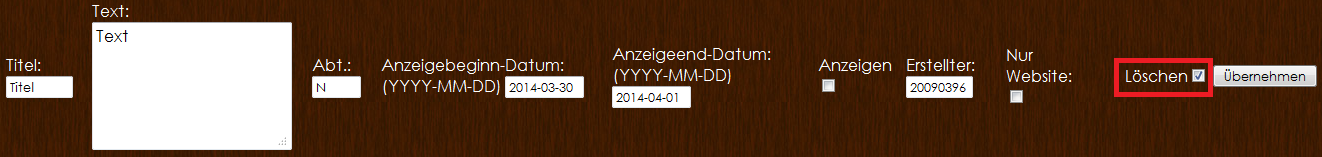
\includegraphics[keepaspectratio=true, width=16cm]{images/screenshots/news_delete.png}
\caption{News löschen}
\label{fig:instr_admin_news_delete}
\end{figure}